\section{Newton-Euler Model Derivation}
\label{s:Winch_Model_Derivation}
The model presented is derived using Newton-Euler methods. Figure \ref{fig:Free_Body_Diagram_MBW} shows the free body diagram of the tractor-winch-sled system. A one dimensional model is used since the dynamics of a heavy, tracked vehicle do not involve aggressive maneuvers and the height of the drawbar hitch is below the vehicle's center of gravity so as to prevent pitching. 
\begin{figure}[tb]
    \centering
    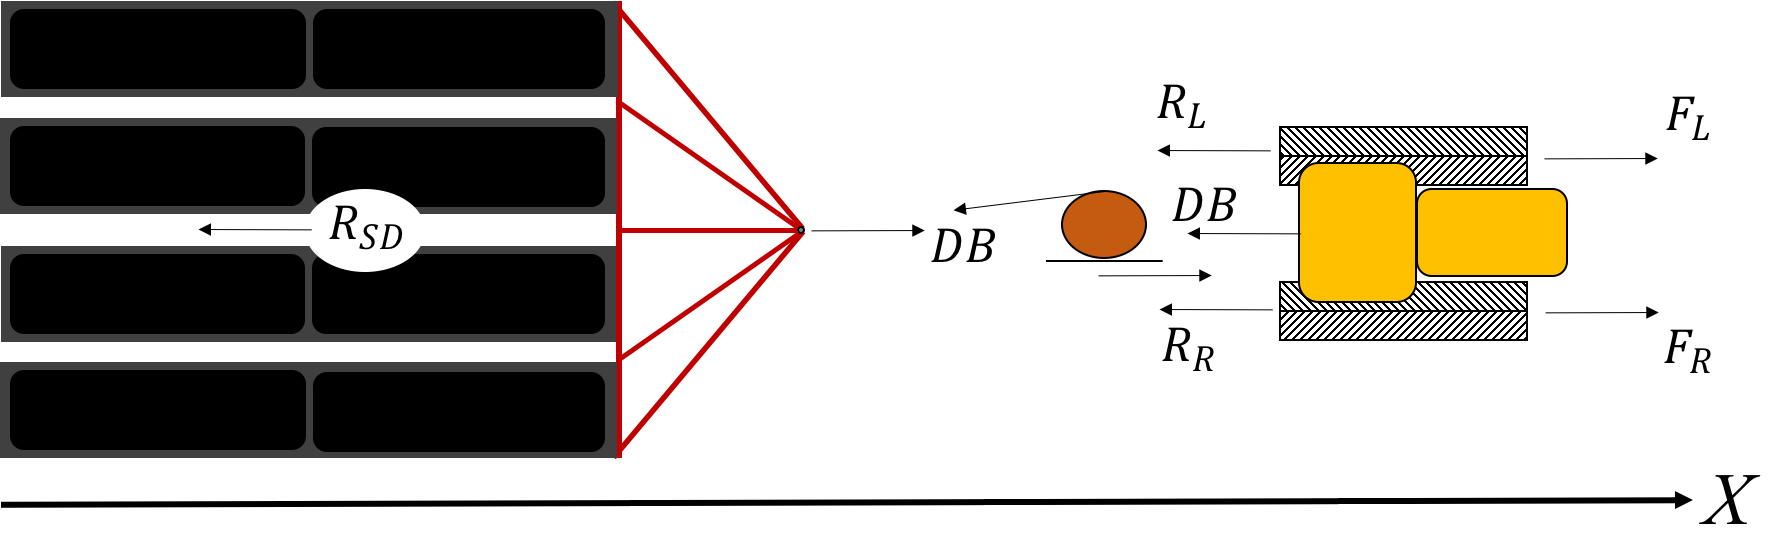
\includegraphics[width = 5in, keepaspectratio]{Free_Body_Diagram_MB_Winch}
    \caption{Free body diagram of the tractor-sled vehicle. The winch is turned sideways for illustration and is colored orange}
    \label{fig:Free_Body_Diagram_MBW}
\end{figure}
Because the cable is incapable of sustaining a compression load and maximum and minimum cable length limitations, this model will have different sets of differential equations that govern its dynamics depending on its current operating condition. A system of this type is called a hybrid system and is said to have hybrid dynamics. These different sets of differental equations will be refered to as phases and are described as follows:
\begin{singlespace}
\centering
\vspace{-10pt}
\begin{enumerate}
    \item Cable in tension, winch is unlocked
    \item Cable in tension, winch is locked
    \item Cable not in tension, winch is unlocked
    \item Cable not in tension, winch is locked
\end{enumerate}
\end{singlespace}

The first phase covered will be where there is tension in the cable and the load is being let out or reeled back in and has not exceeded minimum or maximum cable length limitaitons. The state vector for this phase is $\mathbf{x}_1 = [v_T, \dot\psi, v_{SD}, DB, \dot\varphi_L, \dot\varphi_R]^T$. The governing differential equations and constraint are given by
\begin{equation}
    v_T = \frac{1}{m_T}(F_R - F_L - R_R - R_L - DB)
\end{equation}
\begin{equation}
    \ddot\psi = \frac{1}{J_W}(- \tau_W + r_WDB - \text{sign}(\dot\psi)\zeta_W\dot\psi)
\end{equation}
\begin{equation}
    \dot v_{SD} = \frac{1}{m_{SD}}(DB - R_{SD})
\end{equation}
\begin{equation}
    \ddot\varphi_L = \frac{1}{J_S}(\tau_L - F_Lr - \zeta\dot\varphi_L)
\end{equation}
\begin{equation}
    \ddot\varphi_R = \frac{1}{J_S}(\tau_R - F_Rr - \zeta\dot\varphi_R)
\end{equation}
\begin{equation}\label{eq:KCN1}
    v_{SD} = \dot{\psi} r_W + v_T
\end{equation}
where $J_W$ is the winch rotational inertia, $\tau_W$ is the winch torque, $\psi$ is the winch angular position, $\dot\psi$ is the winch angular velocity, $\zeta_W$ is the winch damping coefficient, and $\psi r_W$ indicates the amount of cable let out by the winch and can only take on nonnegative values. The kinematic constraint in equation \ref{eq:KCN1} is differentiated in order to solve for $v_T$, $\ddot\psi$, $v_{SD}$, and $DB$.
\begin{equation}
    \dot v_{SD} = \ddot{\psi} r_W + \dot v_T
\end{equation}
These derivatives of the state vector can be solved for as a linear system of equations and seperated into the mass matrix $\mathbf{M}_1$ and force vector $\mathbf{\Gamma}_1$.
\begin{equation}
    \mathbf{\dot x_1} = \mathbf{M}_1^{-1}\mathbf{\Gamma}_1(\mathbf{x_1},\mathbf{u}) \quad s.t. \quad DB\geq0, \psi\geq0, \psi r_W \leq L_C
\end{equation}
\begin{equation}
     \mathbf{M}_1 = \begin{bmatrix} J_S & 0 & 0 & 0 & 0 & 0\\ 0 & J_S & 0 & 0 & 0 & 0 \\ 0 & 0 & m_T & 0 & 0 & 1 \\ 0 & 0 & 0 & J_W & 0 & -r_W \\ 0 & 0 & 0 & 0 & m_S & -1 \\ 0 & 0 & -1 & r_W & 1 & 0 \end{bmatrix}
\end{equation}
\begin{equation}
     \mathbf{\Gamma}_1 = \begin{bmatrix} \tau_L - F_Lr - \zeta\dot\varphi_L \\ \tau_R - F_Rr - \zeta\dot\varphi_R \\ F_L + F_R - R_L - R_R \\ -\tau_W - \text{sign}(\dot\psi)\zeta_W\dot\psi \\ -R_{SD} \\ 0 \end{bmatrix}
\end{equation}

The second operating phase governs the dynamics of the tractor sled vehicle when there is tension in the cable and locked. This condition is met when the winch has let out the payload to its maximum length, reeled in the towed load, or has braked to stop the release of cable length. The state vector in this phase is $\mathbf{x}_2 = [v_T, v_{SD}, DB, \dot\varphi_L, \dot\varphi_R]^T$. The governing differential equations are 
\begin{equation}
    \mathbf{\dot x_2} = \mathbf{M}_2^{-1}\mathbf{\Gamma}_2(\mathbf{x_2},\mathbf{u}) \quad s.t. \quad DB\geq0, \psi\geq0, \psi r_W \leq L_C, \dot\psi = 0
\end{equation}
\begin{equation}
     \mathbf{M}_2 = \begin{bmatrix} J_S & 0 & 0 & 0 & 0 \\ 0 & J_S & 0 & 0 & 0 \\ 0 & 0 & m_T & 0 & 1 \\ 0 & 0 & 0 & m_S & -1 \\ 0 & 0 & -1 & 1 & 0 \end{bmatrix}
\end{equation}
\begin{equation}
     \mathbf{\Gamma}_3 = \begin{bmatrix} \tau_L - F_Lr - \zeta\dot\varphi_L \\ \tau_R - F_Rr - \zeta\dot\varphi_R \\ F_L + F_R - R_L - R_R \\ -R_{SD} \\ 0 \end{bmatrix}
\end{equation}

The third phase governs the dynamics when there is no tension in the cable and the winch is unlocked. This is an undesirable phase for operation but is included for model completeness. The state vector in this phase is $\mathbf{x}_3 = [v_T, \dot\psi, v_{SD}, \dot\varphi_L, \dot\varphi_R]^T$. The governing differential equations and constraint are given by
\begin{equation}
    \mathbf{\dot x_3} = \mathbf{M}_3^{-1}\mathbf{\Gamma}_3(\mathbf{x_3},\mathbf{u}) \quad s.t. \quad DB\geq0, \psi\geq0, \psi r_W \leq L_C
\end{equation}
\begin{equation}
     \mathbf{M}_3 = \begin{bmatrix} J_S & 0 & 0 & 0 & 0 \\ 0 & J_S & 0 & 0 & 0  \\ 0 & 0 & m_T & 0 & 0  \\ 0 & 0 & 0 & J_W & 0  \\ 0 & 0 & 0 & 0 & m_S \end{bmatrix}
\end{equation}
\begin{equation}
     \mathbf{\Gamma}_3 = \begin{bmatrix} \tau_L - F_Lr - \zeta\dot\varphi_L \\ \tau_R - F_Rr - \zeta\dot\varphi_R \\ F_L + F_R - R_L - R_R \\ -\tau_W - \text{sign}(\dot\psi)\zeta_W\dot\psi \\ -R_{SD} \end{bmatrix}
\end{equation}

The fourth phase governs the dynamics when there is no tension in the cable and the winch is locked. This is a second undesirable phase for operation but is also included for completeness. The state vector for this phase is $\mathbf{x}_4 = [v_T, v_S, \dot\varphi_L, \dot\varphi_R]^T$. The governing differential equations are
\begin{equation}
    \mathbf{\dot x_4} = \mathbf{M}_4^{-1}\mathbf{\Gamma}_4(\mathbf{x_4},\mathbf{u}) \quad s.t. \quad DB\geq0, \psi\geq0, \psi r_W \leq L_C, \dot\psi = 0
\end{equation}
\begin{equation}
     \mathbf{M}_3 = \begin{bmatrix} J_S & 0 & 0 & 0 \\ 0 & J_S & 0 & 0 \\ 0 & 0 & m_T & 0 \\  0 & 0 & 0 & m_S \end{bmatrix}
\end{equation}
\begin{equation}
     \mathbf{\Gamma}_3 = \begin{bmatrix} \tau_L - F_Lr - \zeta\dot\varphi_L \\ \tau_R - F_Rr - \zeta\dot\varphi_R \\ F_L + F_R - R_L - R_R \\ -R_{SD} \end{bmatrix}
\end{equation}

It is important to capture all these operating modes for completeness and full understanding of the system dynamics. Transitions between modes and the events that trigger them are discussed in a subsequent section. However, the equations governing the hydraulics must be derived first before developing a state machine for the hybrid dynamics